\documentclass[]{book}
\usepackage{lmodern}
\usepackage{amssymb,amsmath}
\usepackage{ifxetex,ifluatex}
\usepackage{fixltx2e} % provides \textsubscript
\ifnum 0\ifxetex 1\fi\ifluatex 1\fi=0 % if pdftex
  \usepackage[T1]{fontenc}
  \usepackage[utf8]{inputenc}
\else % if luatex or xelatex
  \ifxetex
    \usepackage{mathspec}
  \else
    \usepackage{fontspec}
  \fi
  \defaultfontfeatures{Ligatures=TeX,Scale=MatchLowercase}
\fi
% use upquote if available, for straight quotes in verbatim environments
\IfFileExists{upquote.sty}{\usepackage{upquote}}{}
% use microtype if available
\IfFileExists{microtype.sty}{%
\usepackage{microtype}
\UseMicrotypeSet[protrusion]{basicmath} % disable protrusion for tt fonts
}{}
\usepackage{hyperref}
\hypersetup{unicode=true,
            pdftitle={An Introduction to R at Met Council},
            pdfauthor={Katie Jolly},
            pdfborder={0 0 0},
            breaklinks=true}
\urlstyle{same}  % don't use monospace font for urls
\usepackage{natbib}
\bibliographystyle{apalike}
\usepackage{color}
\usepackage{fancyvrb}
\newcommand{\VerbBar}{|}
\newcommand{\VERB}{\Verb[commandchars=\\\{\}]}
\DefineVerbatimEnvironment{Highlighting}{Verbatim}{commandchars=\\\{\}}
% Add ',fontsize=\small' for more characters per line
\usepackage{framed}
\definecolor{shadecolor}{RGB}{248,248,248}
\newenvironment{Shaded}{\begin{snugshade}}{\end{snugshade}}
\newcommand{\KeywordTok}[1]{\textcolor[rgb]{0.13,0.29,0.53}{\textbf{#1}}}
\newcommand{\DataTypeTok}[1]{\textcolor[rgb]{0.13,0.29,0.53}{#1}}
\newcommand{\DecValTok}[1]{\textcolor[rgb]{0.00,0.00,0.81}{#1}}
\newcommand{\BaseNTok}[1]{\textcolor[rgb]{0.00,0.00,0.81}{#1}}
\newcommand{\FloatTok}[1]{\textcolor[rgb]{0.00,0.00,0.81}{#1}}
\newcommand{\ConstantTok}[1]{\textcolor[rgb]{0.00,0.00,0.00}{#1}}
\newcommand{\CharTok}[1]{\textcolor[rgb]{0.31,0.60,0.02}{#1}}
\newcommand{\SpecialCharTok}[1]{\textcolor[rgb]{0.00,0.00,0.00}{#1}}
\newcommand{\StringTok}[1]{\textcolor[rgb]{0.31,0.60,0.02}{#1}}
\newcommand{\VerbatimStringTok}[1]{\textcolor[rgb]{0.31,0.60,0.02}{#1}}
\newcommand{\SpecialStringTok}[1]{\textcolor[rgb]{0.31,0.60,0.02}{#1}}
\newcommand{\ImportTok}[1]{#1}
\newcommand{\CommentTok}[1]{\textcolor[rgb]{0.56,0.35,0.01}{\textit{#1}}}
\newcommand{\DocumentationTok}[1]{\textcolor[rgb]{0.56,0.35,0.01}{\textbf{\textit{#1}}}}
\newcommand{\AnnotationTok}[1]{\textcolor[rgb]{0.56,0.35,0.01}{\textbf{\textit{#1}}}}
\newcommand{\CommentVarTok}[1]{\textcolor[rgb]{0.56,0.35,0.01}{\textbf{\textit{#1}}}}
\newcommand{\OtherTok}[1]{\textcolor[rgb]{0.56,0.35,0.01}{#1}}
\newcommand{\FunctionTok}[1]{\textcolor[rgb]{0.00,0.00,0.00}{#1}}
\newcommand{\VariableTok}[1]{\textcolor[rgb]{0.00,0.00,0.00}{#1}}
\newcommand{\ControlFlowTok}[1]{\textcolor[rgb]{0.13,0.29,0.53}{\textbf{#1}}}
\newcommand{\OperatorTok}[1]{\textcolor[rgb]{0.81,0.36,0.00}{\textbf{#1}}}
\newcommand{\BuiltInTok}[1]{#1}
\newcommand{\ExtensionTok}[1]{#1}
\newcommand{\PreprocessorTok}[1]{\textcolor[rgb]{0.56,0.35,0.01}{\textit{#1}}}
\newcommand{\AttributeTok}[1]{\textcolor[rgb]{0.77,0.63,0.00}{#1}}
\newcommand{\RegionMarkerTok}[1]{#1}
\newcommand{\InformationTok}[1]{\textcolor[rgb]{0.56,0.35,0.01}{\textbf{\textit{#1}}}}
\newcommand{\WarningTok}[1]{\textcolor[rgb]{0.56,0.35,0.01}{\textbf{\textit{#1}}}}
\newcommand{\AlertTok}[1]{\textcolor[rgb]{0.94,0.16,0.16}{#1}}
\newcommand{\ErrorTok}[1]{\textcolor[rgb]{0.64,0.00,0.00}{\textbf{#1}}}
\newcommand{\NormalTok}[1]{#1}
\usepackage{longtable,booktabs}
\usepackage{graphicx,grffile}
\makeatletter
\def\maxwidth{\ifdim\Gin@nat@width>\linewidth\linewidth\else\Gin@nat@width\fi}
\def\maxheight{\ifdim\Gin@nat@height>\textheight\textheight\else\Gin@nat@height\fi}
\makeatother
% Scale images if necessary, so that they will not overflow the page
% margins by default, and it is still possible to overwrite the defaults
% using explicit options in \includegraphics[width, height, ...]{}
\setkeys{Gin}{width=\maxwidth,height=\maxheight,keepaspectratio}
\IfFileExists{parskip.sty}{%
\usepackage{parskip}
}{% else
\setlength{\parindent}{0pt}
\setlength{\parskip}{6pt plus 2pt minus 1pt}
}
\setlength{\emergencystretch}{3em}  % prevent overfull lines
\providecommand{\tightlist}{%
  \setlength{\itemsep}{0pt}\setlength{\parskip}{0pt}}
\setcounter{secnumdepth}{5}
% Redefines (sub)paragraphs to behave more like sections
\ifx\paragraph\undefined\else
\let\oldparagraph\paragraph
\renewcommand{\paragraph}[1]{\oldparagraph{#1}\mbox{}}
\fi
\ifx\subparagraph\undefined\else
\let\oldsubparagraph\subparagraph
\renewcommand{\subparagraph}[1]{\oldsubparagraph{#1}\mbox{}}
\fi

%%% Use protect on footnotes to avoid problems with footnotes in titles
\let\rmarkdownfootnote\footnote%
\def\footnote{\protect\rmarkdownfootnote}

%%% Change title format to be more compact
\usepackage{titling}

% Create subtitle command for use in maketitle
\providecommand{\subtitle}[1]{
  \posttitle{
    \begin{center}\large#1\end{center}
    }
}

\setlength{\droptitle}{-2em}

  \title{An Introduction to R at Met Council}
    \pretitle{\vspace{\droptitle}\centering\huge}
  \posttitle{\par}
    \author{Katie Jolly}
    \preauthor{\centering\large\emph}
  \postauthor{\par}
      \predate{\centering\large\emph}
  \postdate{\par}
    \date{2019-08-07}

\usepackage{booktabs}

\begin{document}
\maketitle

{
\setcounter{tocdepth}{1}
\tableofcontents
}
\chapter{Welcome!}\label{welcome}

This book is meant to be a reference for before, during, and after the
in-person session on August 14. It is not comprehensive, but should
serve as a way to help illustrate the different concepts. My hope is
that at the end of it, everyone will be able to read in data, clean and
wrangle it, plot it, and do some simple analysis.

R is a powerful language for statistical analysis and data communication
and we will only get to the surface of everything today. For example,
this map was map entirely with R (as was this book)!

\includegraphics[width=700px]{https://timogrossenbacher.ch/wp-content/uploads/2016/12/tm-final-map-1}

Notes:

\begin{enumerate}
\def\labelenumi{\arabic{enumi}.}
\item
  If you find typos, errors, or clarity issues, please let me know!
\item
  If you want to share this resource (or happen upon it on the internet)
  feel free to share it, I just ask that you credit properly (whether
  that is me or someone I've credited).
\end{enumerate}

\chapter{Installing R and RStudio}\label{setup}

R is the underlying language while RStudio is typically how you will
interact with it. RStudio is an integrated development environment (IDE)
that is generally considered to be one of the best available. It's also
entirely open source and free (unless you want special features) which
is unique among IDEs of its quality. The IDE means that rather than just
being a place for you to write code, ``it includes a console,
syntax-highlighting editor that supports direct code execution, as well
as tools for plotting, history, debugging and workspace management''
(RStudio). In short, this means it makes your code-writing so much
smoother.

\section{RStudio Cloud}\label{rstudio-cloud}

In this workshop, we will be using the
\href{https://rstudio.cloud/}{RStudio cloud} option. I don't recommend
this for long-term use, but it's an awesome resource that makes learning
R \href{https://rstudio.cloud/learn/guide}{easier} and
\href{https://www.causeweb.org/cause/sites/default/files/eCOTS\%202018\%20-\%20Frictionless\%20onboarding\%20to\%20data\%20science\%20with\%20RStudio\%20Cloud.pdf}{less
dependent} on software installation. Each project is allocated 1GB of
RAM which is fine for this workshop, but is not enough for joining large
datasets or fitting complicated models.

To create your cloud account, go to the
\href{https://rstudio.cloud/}{sign-up page}. Click ``Get Started'' and
enter credentials for yourself.

Once you're logged in, your workspace should look something like this:

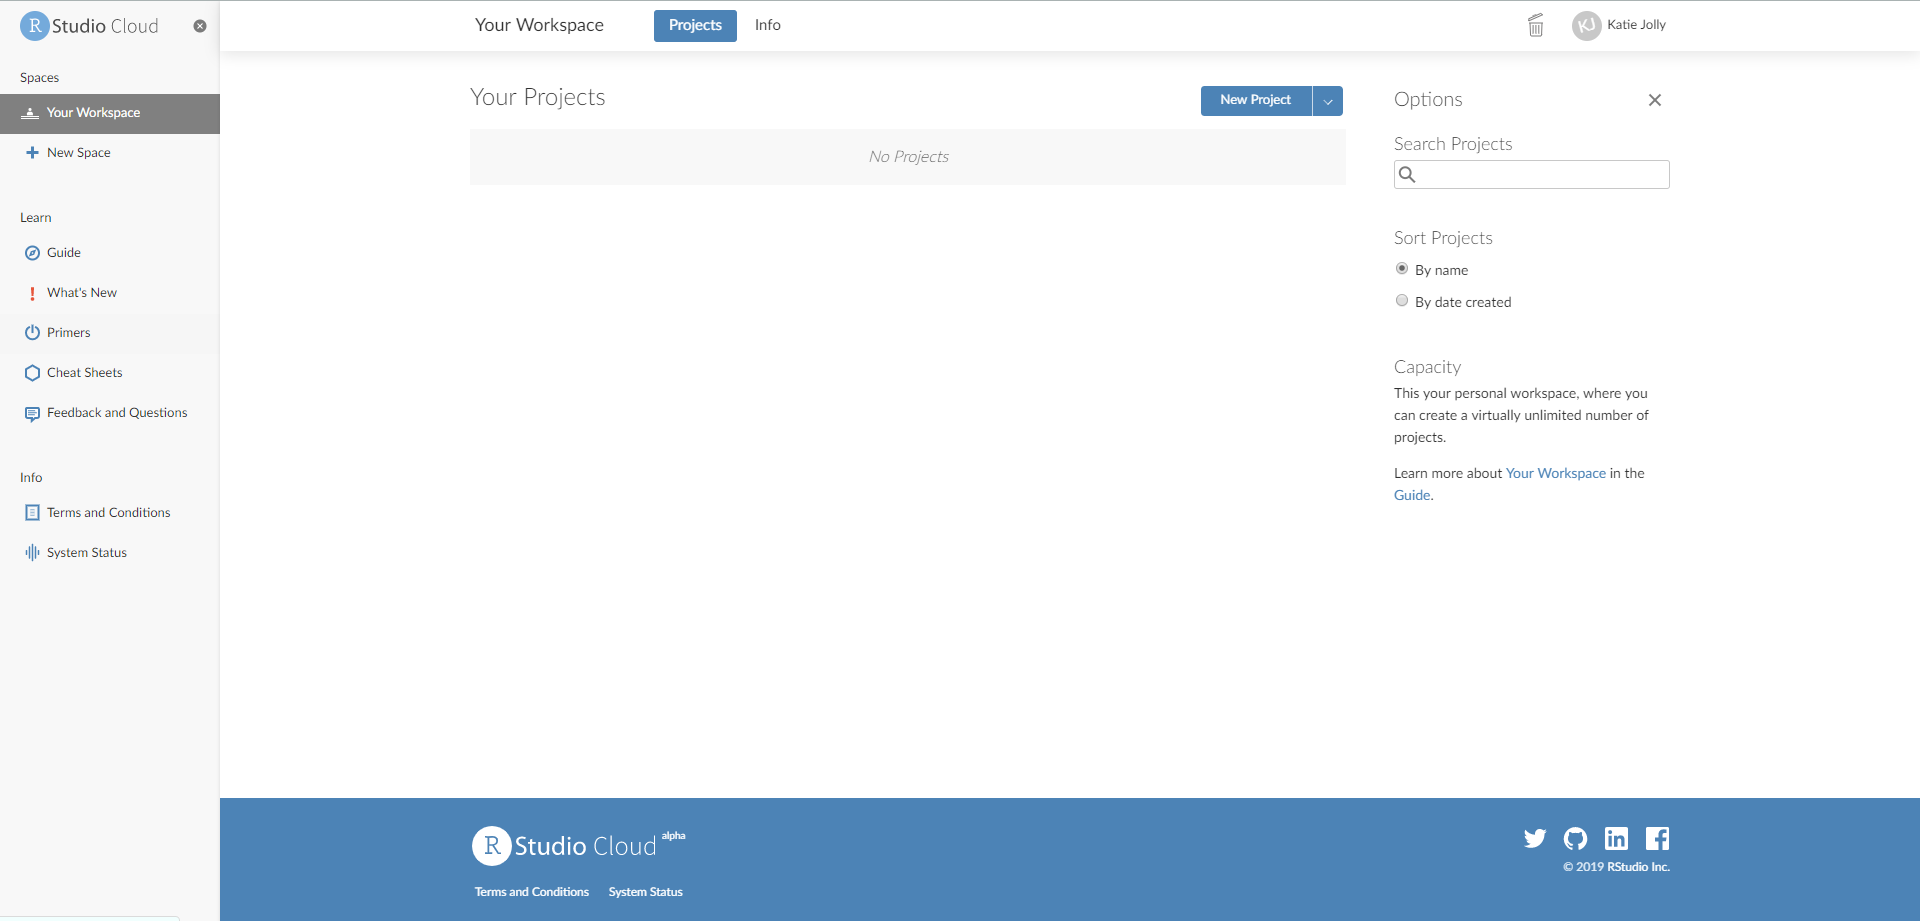
\includegraphics[width=26.67in]{images/rstudiocloud}

\section{RStudio Desktop}\label{rstudio-desktop}

In order to run RStudio on your desktop, you should have
\href{https://cran.r-project.org/mirrors.html}{R} and
\href{https://www.rstudio.com/products/rstudio/download/}{RStudio
Desktop} downloaded, \emph{in that order}.

Here is one guide to walk you through the process:
\url{https://www.ics.uci.edu/~sternh/courses/210/InstallingRandRStudio.pdf}

Note that you should just download the most recent version, the version
numbers in that document are likely out of date.

Once you have both installed, open RStudio and see if it looks like this
(minor deviations are totally fine):

\includegraphics[width=600px]{https://i1.wp.com/www.bytemining.com/wp-content/uploads/2011/03/rstudio}

If you have any questions or run into issues, feel free to stop by my
cube or email me!

\chapter{R Projects}\label{r-projects}

When working on an analysis with R, the recommended workflow is to use
\href{https://r4ds.had.co.nz/workflow-projects.html}{R Projects}. This
is also called
\href{https://www.tidyverse.org/articles/2017/12/workflow-vs-script/}{``project-oriented
workflow''} in some other tutorials.

Projects are nice because they keep all of the data, code, writing, etc.
for a particular task in one place. You don't have to worry about
working directories and reproducibility is more straightforward. It
allows you to use relative versus absolute pathnames, this is awesome
when working with collaborators.

Let's make a project for this workshop!

\section{Set up your project: Cloud}\label{set-up-your-project-cloud}

In your RStudio cloud workspace, click the \texttt{New\ Project} button
to start a project. Once it is open, you can name it by
\texttt{Untitled\ Project} where it says
\texttt{Your\ Workspace/Untitled\ Project} at the top of the screen.
Name it something short but meaningful with no spaces or special
characters except \texttt{-} or \texttt{\_}.

\section{Set up your project:
Desktop}\label{set-up-your-project-desktop}

In the upper right corner of your RStudio window, you'll see
\texttt{Project:\ (None)}. Click on that, then select
\texttt{New\ Project...}. Next select \texttt{New\ Directory}.

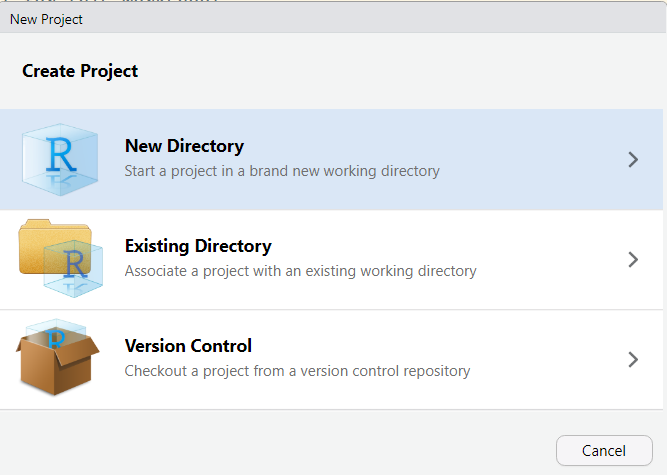
\includegraphics[width=9.26in]{images/03-03-newproject}

Then select \texttt{New\ Project} from the list of options.

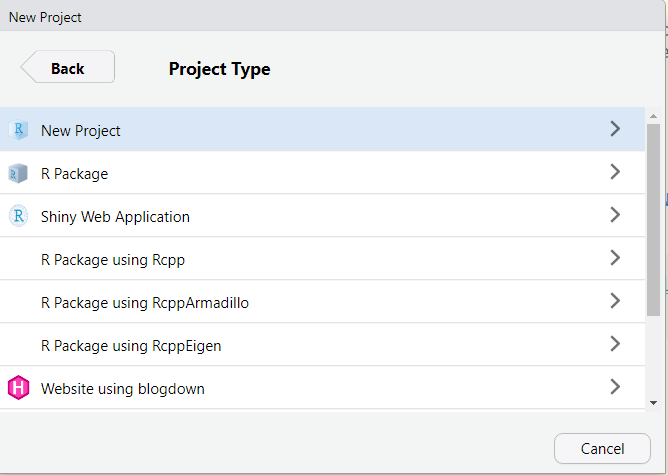
\includegraphics[width=9.28in]{images/03-01-newproject}

Then you can name your project (think of it as naming the folder where
you'll keep all of your work). I like to include the date in my file
names as well. The second part
(\texttt{Create\ project\ as\ a\ subdirectory\ of:}) is where you want
this folder to live on your computer. The default for Windows is your
Documents/ folder.

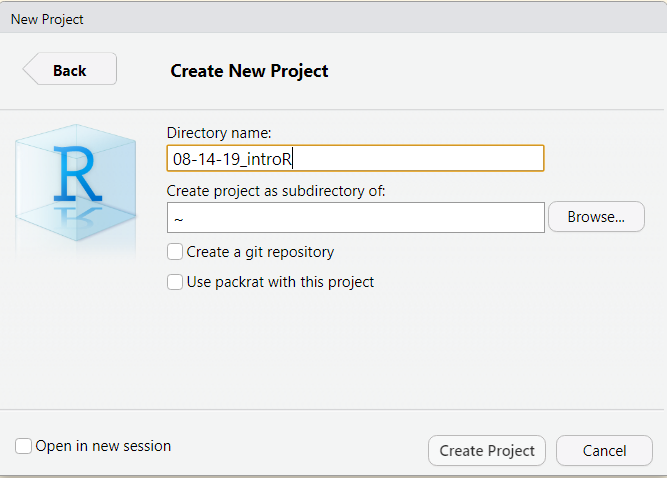
\includegraphics[width=9.26in]{images/03-02-newproject}

Once you've done that, click \texttt{Create\ Project}. You should now
see your current project name in the corner where before you saw
\texttt{Project:\ (None)}.

\chapter{Writing R code}\label{writing-r-code}

There are three main places to write R code while using RStudio. In
order of complexity, they are: the console, R scripts, and R markdown.

\section{The console}\label{the-console}

The console should be thought of as scratch paper. It's a way to test
code before writing it in a document. It's also nice for code that you
only need to run once, like installing a package.

\subsection{Try it out}\label{try-it-out}

\begin{itemize}
\item
  Type \texttt{3+2} and hit enter
\item
  Type \texttt{x\ \textless{}-\ 3+2} and hit enter
\item
  Then, type \texttt{x} and hit enter
\end{itemize}

What did you get back when you typed \texttt{x} into the console?

\begin{itemize}
\tightlist
\item
  Type \texttt{x\ *\ 4} and hit enter
\end{itemize}

What happened now?

\subsection{R objects}\label{r-objects}

R stores information in \textbf{objects}, or variables.

We created an object called \texttt{x} by naming it and assigning it
with the \texttt{\textless{}-} function to the value \texttt{3+2}. You
may also see people write \texttt{x\ =\ 3+2} but that is less common.

Object names should be short and meaningful. They cannot start with a
number and the only special characters allowed are \texttt{.} and
\texttt{\_}. Names are also \textbf{case sensitive}, as is all R code.
Certain words have special meanings and cannot be used as object names.
These include words like \texttt{if} and \texttt{else} because they have
other meanings in R.

\begin{Shaded}
\begin{Highlighting}[]
\ControlFlowTok{if}\NormalTok{ <-}\StringTok{ }\DecValTok{3}\OperatorTok{+}\DecValTok{2}
\end{Highlighting}
\end{Shaded}

\begin{verbatim}
## Error: <text>:1:4: unexpected assignment
## 1: if <-
##        ^
\end{verbatim}

It won't let us create the variable because it's an off-limits name.

As a matter of style, it is recommended to:

\begin{itemize}
\item
  Use nouns
\item
  Avoid using \texttt{.} in names
\item
  Avoid using function names, even when technically allowed (this will
  become easier with time as you learn more function names)
\item
  Pick a style and go with it
\end{itemize}

For example, I prefer using \texttt{\_} in my object names instead of
\texttt{camelCase}. If you want to learn more about style, consider
reading the guides written by
\href{https://google.github.io/styleguide/Rguide.xml}{Google} or the
\href{https://style.tidyverse.org/}{Tidyverse packages} later.

\section{R scripts}\label{r-scripts}

R scripts allow you to save the code that you write to run again later.
They are essentially a document meant to read code. Let's make one.

Go to \textbf{File \textgreater{} New File \textgreater{} R Script} or
\textbf{ctrl + shift + N}.

Save your new R script in a new folder called \texttt{R} within your
project folder.

On the first line, create an object that is assigned to your name. In R,
characters (words) need to be surrounded by quotes. Numbers do not.

First, try without quotes. To run this either press the run button at
the top of the script or press \textbf{ctrl + enter} when your cursor is
on the line you want to run.

\begin{Shaded}
\begin{Highlighting}[]
\NormalTok{name <-}\StringTok{ }\NormalTok{Katie}
\end{Highlighting}
\end{Shaded}

\begin{verbatim}
## Error in eval(expr, envir, enclos): object 'Katie' not found
\end{verbatim}

It's looking for an object called Katie. Why?

In R, variable names do not need quotes. This is how they are
distinguished visually from character data.

Let's try again.

\begin{Shaded}
\begin{Highlighting}[]
\NormalTok{name <-}\StringTok{ "Katie"}
\end{Highlighting}
\end{Shaded}

\subsection{Comments}\label{comments}

Whenever you're writing code, think of it as writing for someone who
isn't you. What this means is that you should leave comments that
explain your thought process. People have differing opinions on what a
good comment is, but it generally shouldn't be something that just
repeats the code. It should be something about why you chose that
function, what you expect to get in your output, issues you had, etc
etc.

In R you can write a comment by having a \texttt{\#} at the beginning of
the line.

In your script, write a comment to yourself about one thing you hope to
be able to do in R after the workshop today.

\section{R markdown}\label{r-markdown}

The third, and most universally useful in my opinion, way to write code
is in an R markdown document. If you've used Jupyter notebooks in
Python, it's a similar idea. R markdown is a way to interweave code,
analysis, output, and prose. The pandoc engine ``knits'' your document
into a Word doc, PDF, or HTML. This book is an HTML file knitted from a
bunch of R markdowns!

Today we will be working in R markdown to save our work and be able to
reference it later.

To create an R markdown, go to \textbf{File \textgreater{} New File
\textgreater{} R Markdown\ldots{}}

Write a title for your document (this is \textbf{not} the same thing as
naming the file), add your name, and select HTML as the output format.

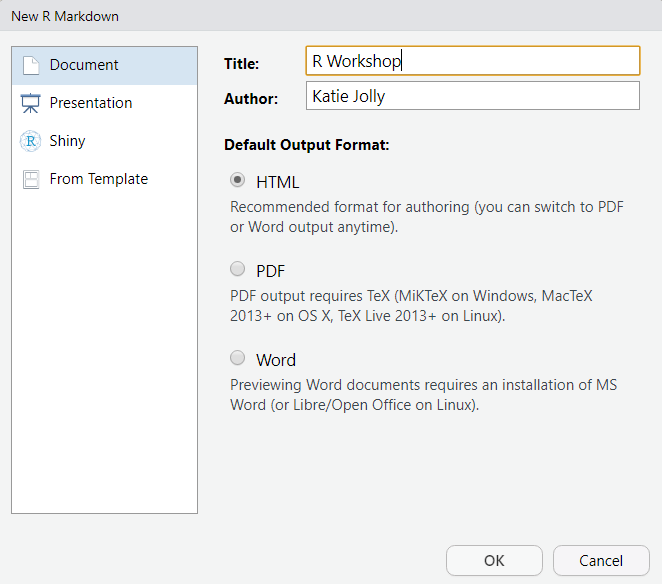
\includegraphics[width=9.19in]{images/03-04-newmarkdown}

Erase everything in your document \textbf{except} the header. This is
the part enclosed by \texttt{-\/-\/-}. But let me know if you
accidentally delete that too! It's not hard to fix. Anything typed just
directly onto the document is plain text. We will write code in
``chunks'' later. There are also nice ways to include HTML elements like
headers and bold text.

\begin{itemize}
\item
  At the top of your document, write a short paragraph about the best
  thing that happened to you last week. Start it with the header
  \texttt{\#\ Best\ part\ of\ last\ week}. The \texttt{\#} in plain text
  indicates a header.
\item
  In your paragraph, use bold text at least once and bullet points at
  least twice. Use the R markdown
  \href{https://www.rstudio.com/wp-content/uploads/2015/02/rmarkdown-cheatsheet.pdf}{cheat
  sheet} to figure out how to do that.
\item
  Next, add this photo to your R markdown:
  \url{https://www.metrotransit.org/Data/Sites/1/media/metro/greenline/metro_greenline_map_031716_web.png}
\end{itemize}

\includegraphics{https://www.metrotransit.org/Data/Sites/1/media/metro/greenline/metro_greenline_map_031716_web.png}

\begin{itemize}
\item
  Finally, insert an R chunk from the top of the document by clicking
  \textbf{Insert \textgreater{} R} or \textbf{ctrl + alt + i}. Type
  \texttt{3\ +\ 4} and then run the code with the green arrow.
\item
  Now, knit your HTML (\emph{Knit}) to see what it looks like!
\end{itemize}

\chapter{Packages}\label{packages}

R as a language on its own is useful, but the open-source nature of R
means that packages can greatly extend its capabilities. Instead of
writing a function for every process, there's a good chance someone else
already has! There are packages for nearly every task you might want to
do in R. If you're an ArcGIS user, one analogy for a package is that it
is similar to extensions like Spatial Analyst. If you want to take a
more literal approach each function of ArcGIS can be thought of like a
package because someone has already taken the time to write that code
and make it generally useful.

For this tutorial, you'll need a few main packages. Type (don't
copy/paste) this code into your \emph{console} (see image below) and
click enter. Click ``OK'' if it prompts you to restart R. This will only
restart the underlying R engine, not your RStudio interface.

\begin{Shaded}
\begin{Highlighting}[]
\KeywordTok{install.packages}\NormalTok{(}\KeywordTok{c}\NormalTok{(}\StringTok{"knitr"}\NormalTok{, }\StringTok{"tidyverse"}\NormalTok{, }\StringTok{"devtools"}\NormalTok{, }\StringTok{"rmarkdown"}\NormalTok{))}
\end{Highlighting}
\end{Shaded}

You can check that your packages installed correctly by loading the
libraries into your R session. Type this into your console and press
enter.

\begin{Shaded}
\begin{Highlighting}[]
\KeywordTok{library}\NormalTok{(knitr)}
\KeywordTok{library}\NormalTok{(tidyverse)}
\KeywordTok{library}\NormalTok{(devtools)}
\KeywordTok{library}\NormalTok{(rmarkdown)}
\end{Highlighting}
\end{Shaded}

If you don't see an error, you're good-to-go.

\begin{center}\includegraphics[width=500px]{http://gsp.humboldt.edu/OLM/R/Images/RStudio_1} \end{center}

\chapter{Reading in Data}\label{reading-in-data}

I am a strong believer in the
\href{https://twitter.com/minebocek/status/1072222447473168389}{cake-first}
approach to teaching/learning R. It emphasizes real-world examples,
interesting data, and visual feedback. Because of that, I like to use
ready-made data packages like \texttt{fivethirtyeight} and talk about
visualization \emph{before} data cleaning.

But I also think reading in data is an important skill so we will talk
about that briefly at the end of today, but not spend too much time on
it. For now, let's eat the cake instead of going out to get the
ingredients. That's more fun anyway.

\section{Data packages}\label{data-packages}

There are a number of packages in R specifically to make data sharing
easier. A few examples are:

\begin{itemize}
\item
  \texttt{fivethirtyeight} to share to data used in their articles
\item
  \texttt{bikedata} to share data about certain bikeshare systems
\item
  \texttt{ecoengine} to share data from the Berkley natural history
  museum
\end{itemize}

We will use the data the MN niceride system. I put the data in a package
so it's easy to use. You can install it by typing
\texttt{install\_github("katiejolly/metcouncilR")} in your console.

\subsection{Try it out}\label{try-it-out-1}

In your R markdown, fill in the following code to load your library:

\begin{Shaded}
\begin{Highlighting}[]
\KeywordTok{___}\NormalTok{(metcouncilR)}
\end{Highlighting}
\end{Shaded}

To pull a particular dataset from this package, we can use the
\texttt{data()} function.

\begin{Shaded}
\begin{Highlighting}[]
\KeywordTok{data}\NormalTok{(}\StringTok{"nice_ride_2018"}\NormalTok{) }\CommentTok{# niceride dataset}
\end{Highlighting}
\end{Shaded}

You should now see it in your global working environment.

I've written documentation for this data that you can see in the help
pane in RStudio.

\begin{Shaded}
\begin{Highlighting}[]
\KeywordTok{help}\NormalTok{(}\StringTok{"nice_ride_2018"}\NormalTok{)}
\end{Highlighting}
\end{Shaded}

There are also a few different ways to get quick summaries of the data.

First, you can check the dimensions to get the number of rows and
columns.

\begin{Shaded}
\begin{Highlighting}[]
\KeywordTok{dim}\NormalTok{(nice_ride_}\DecValTok{2018}\NormalTok{)}
\end{Highlighting}
\end{Shaded}

\begin{verbatim}
## [1] 412423     16
\end{verbatim}

What function would you use to get just the number of columns? (Google
it.)

\begin{Shaded}
\begin{Highlighting}[]
\KeywordTok{___}\NormalTok{(nice_ride_}\DecValTok{2018}\NormalTok{)}
\end{Highlighting}
\end{Shaded}

We can also print the first 6 rows of the data with the \texttt{head()}
function.

\begin{Shaded}
\begin{Highlighting}[]
\KeywordTok{head}\NormalTok{(nice_ride_}\DecValTok{2018}\NormalTok{)}
\end{Highlighting}
\end{Shaded}

\begin{verbatim}
## # A tibble: 6 x 16
##   tripduration start_time          end_time            start_station_id
##          <dbl> <dttm>              <dttm>                         <dbl>
## 1         1373 2018-04-24 16:03:04 2018-04-24 16:25:57              170
## 2         1730 2018-04-24 16:38:40 2018-04-24 17:07:31                2
## 3          547 2018-04-24 17:51:10 2018-04-24 18:00:17               13
## 4          856 2018-04-24 18:50:05 2018-04-24 19:04:22               94
## 5          455 2018-04-25 08:49:05 2018-04-25 08:56:40               13
## 6         1557 2018-04-27 11:57:03 2018-04-27 12:23:01               43
## # ... with 12 more variables: start_station_name <chr>,
## #   start_station_latitude <dbl>, start_station_longitude <dbl>,
## #   end_station_id <dbl>, end_station_name <chr>,
## #   end_station_latitude <dbl>, end_station_longitude <dbl>, bikeid <dbl>,
## #   usertype <chr>, birth_year <dbl>, gender <dbl>, bike_type <chr>
\end{verbatim}

How can we modify this code to print the first \textbf{10} rows instead?
(hint: \texttt{help(head)} to see the documentation)

\begin{Shaded}
\begin{Highlighting}[]
\KeywordTok{head}\NormalTok{(nice_ride_}\DecValTok{2018}\NormalTok{, }\DataTypeTok{__ =}\NormalTok{ ___)}
\end{Highlighting}
\end{Shaded}

We can also just get a summary of each variable.

\begin{Shaded}
\begin{Highlighting}[]
\KeywordTok{summary}\NormalTok{(nice_ride_}\DecValTok{2018}\NormalTok{)}
\end{Highlighting}
\end{Shaded}

\begin{verbatim}
##   tripduration        start_time                 
##  Min.   :      61   Min.   :2018-04-12 08:49:49  
##  1st Qu.:     434   1st Qu.:2018-06-08 15:49:25  
##  Median :     808   Median :2018-07-18 10:10:37  
##  Mean   :    3825   Mean   :2018-07-20 04:58:26  
##  3rd Qu.:    1548   3rd Qu.:2018-08-27 22:36:27  
##  Max.   :11136253   Max.   :2018-11-17 23:51:45  
##                                                  
##     end_time                   start_station_id start_station_name
##  Min.   :2018-04-12 09:31:20   Min.   :  2.0    Length:412423     
##  1st Qu.:2018-06-08 16:27:45   1st Qu.: 37.0    Class :character  
##  Median :2018-07-18 10:56:49   Median : 94.0    Mode  :character  
##  Mean   :2018-07-20 06:02:11   Mean   :103.5                      
##  3rd Qu.:2018-08-28 06:23:01   3rd Qu.:171.0                      
##  Max.   :2018-12-03 09:33:56   Max.   :226.0                      
##                                NA's   :13443                      
##  start_station_latitude start_station_longitude end_station_id 
##  Min.   :44.89          Min.   :-93.33          Min.   :  2.0  
##  1st Qu.:44.96          1st Qu.:-93.27          1st Qu.: 38.0  
##  Median :44.97          Median :-93.26          Median : 95.0  
##  Mean   :44.97          Mean   :-93.25          Mean   :103.7  
##  3rd Qu.:44.98          3rd Qu.:-93.23          3rd Qu.:170.0  
##  Max.   :45.04          Max.   :-93.08          Max.   :611.0  
##                                                 NA's   :13443  
##  end_station_name   end_station_latitude end_station_longitude
##  Length:412423      Min.   :44.75        Min.   :-93.38       
##  Class :character   1st Qu.:44.96        1st Qu.:-93.28       
##  Mode  :character   Median :44.97        Median :-93.26       
##                     Mean   :44.97        Mean   :-93.25       
##                     3rd Qu.:44.98        3rd Qu.:-93.23       
##                     Max.   :45.04        Max.   :-93.08       
##                                                               
##      bikeid       usertype           birth_year       gender      
##  Min.   :   2   Length:412423      Min.   :1911   Min.   :0.0000  
##  1st Qu.: 530   Class :character   1st Qu.:1969   1st Qu.:0.0000  
##  Median :1056   Mode  :character   Median :1969   Median :1.0000  
##  Mean   :1092                      Mean   :1976   Mean   :0.7054  
##  3rd Qu.:1627                      3rd Qu.:1986   3rd Qu.:1.0000  
##  Max.   :3341                      Max.   :2000   Max.   :2.0000  
##                                                                   
##   bike_type        
##  Length:412423     
##  Class :character  
##  Mode  :character  
##                    
##                    
##                    
## 
\end{verbatim}

But you'll notice these aren't that meaningful for the character
variables. Another way we can extract information about a variable is to
use the \texttt{\$} operator. To just pull out one variable from a
dataset, you would write \texttt{data\$variable}. We can use this syntax
to make a table of the user types.

\begin{Shaded}
\begin{Highlighting}[]
\KeywordTok{table}\NormalTok{(nice_ride_}\DecValTok{2018}\OperatorTok{$}\NormalTok{usertype)}
\end{Highlighting}
\end{Shaded}

\begin{verbatim}
## 
##   Customer Subscriber 
##     290947     121476
\end{verbatim}

\subsection{Practice}\label{practice}

\begin{enumerate}
\def\labelenumi{\arabic{enumi}.}
\item
  How many of the users were female?
\item
  What was the longest trip duration?
\item
  Looking at the documentation, why might an end station name be empty?
\item
  Looking at the documentation, what is the unit of the
  \texttt{tripduration} variable empty?
\item
  What kinds of trips are excluded from this data?
\end{enumerate}

\chapter{Visualization}\label{visualization}

We will start with univariate visualization to learn the syntax, and
then later move into more complex multivariate visualizations.

R has some built-in plotting ability. It's good to recognize the syntax,
but it's not super common to see ``in-the-wild'' these days.

\section{Base R plotting}\label{base-r-plotting}

R can make histograms:

\begin{Shaded}
\begin{Highlighting}[]
\KeywordTok{hist}\NormalTok{(nice_ride_}\DecValTok{2018}\OperatorTok{$}\NormalTok{tripduration) }\CommentTok{# this one isn't great because the distribution is so skewed}
\end{Highlighting}
\end{Shaded}

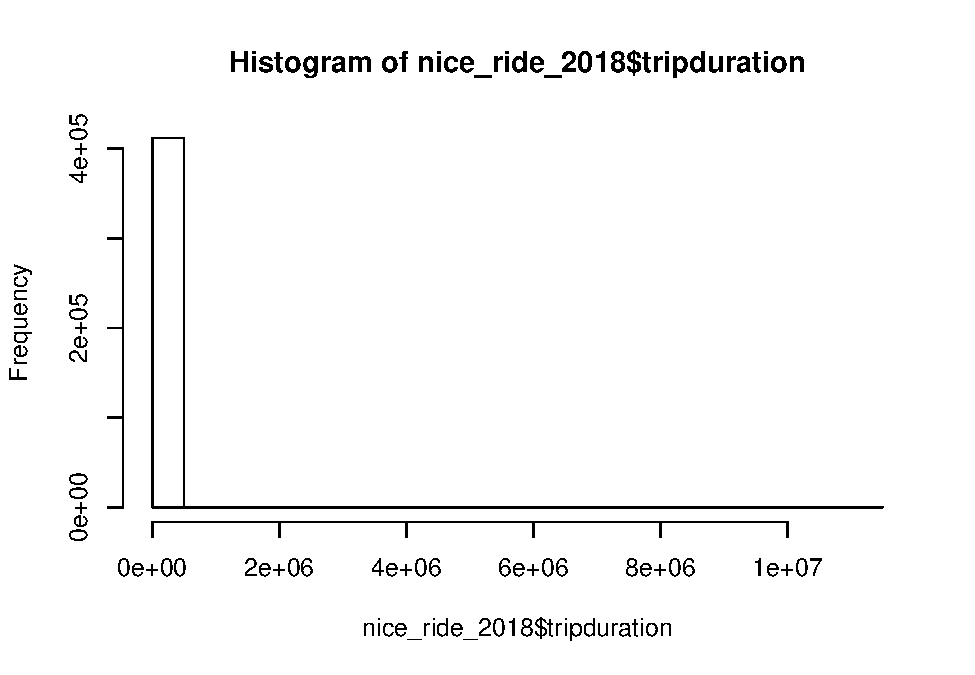
\includegraphics{met-council-introR_files/figure-latex/unnamed-chunk-26-1.pdf}

And bar plots:

\begin{Shaded}
\begin{Highlighting}[]
\KeywordTok{barplot}\NormalTok{(}\KeywordTok{table}\NormalTok{(nice_ride_}\DecValTok{2018}\OperatorTok{$}\NormalTok{usertype), }\DataTypeTok{main =} \StringTok{"User Type"}\NormalTok{) }
\end{Highlighting}
\end{Shaded}

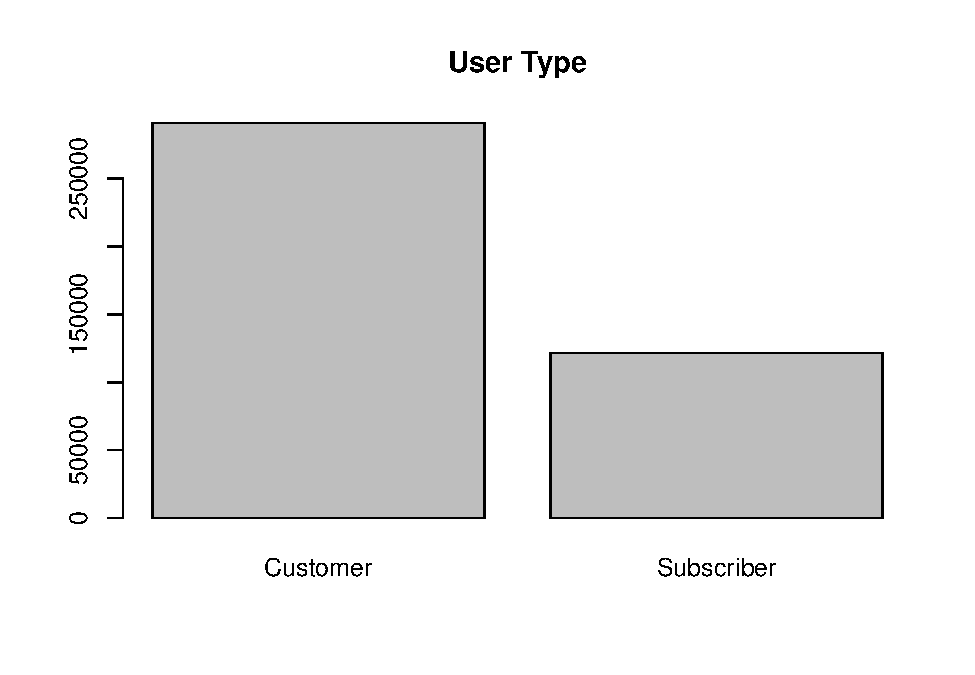
\includegraphics{met-council-introR_files/figure-latex/unnamed-chunk-27-1.pdf}

\begin{Shaded}
\begin{Highlighting}[]
\KeywordTok{barplot}\NormalTok{(}\KeywordTok{table}\NormalTok{(nice_ride_}\DecValTok{2018}\OperatorTok{$}\NormalTok{bike_type), }\DataTypeTok{main =} \StringTok{"Bike Type"}\NormalTok{)}
\end{Highlighting}
\end{Shaded}

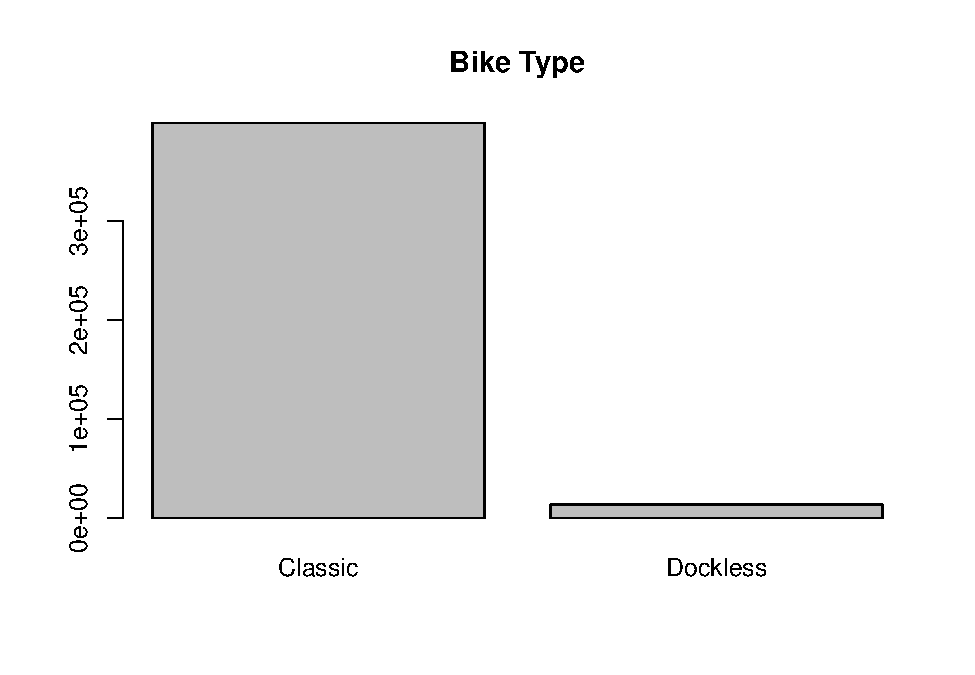
\includegraphics{met-council-introR_files/figure-latex/unnamed-chunk-27-2.pdf}

But base R plots are hard to customize and an inconsistent syntax.
There's general agreement that they're not the best way to plot data in
R so we aren't going to talk much about it.

\section{ggplot2}\label{ggplot2}

\texttt{ggplot2} is without competiton in the graphics in R world. Not
only is it the most popular plotting package, it's one of the most
popular packages, period. It is included in the tidyverse, which we
already loaded. Part of the strength of ggplot is its customizability.
You can create beautiful plots all in R with it. For example, the map on
the cover of this book was
\href{https://timogrossenbacher.ch/2016/12/beautiful-thematic-maps-with-ggplot2-only/}{made
with ggplot}.

\includegraphics[width=700px]{https://timogrossenbacher.ch/wp-content/uploads/2016/12/tm-final-map-1}

ggplot uses the ``grammar of graphics'' to layer information onto plots.
Each plot has the same general structure which makes it easy once you
learn the structure.

\subsection{Categorical data}\label{categorical-data}

For example, let's recreate the bar plot of user types from above.

We will layer on the information in stages.

\textbf{Stage 1}: The plotting canvas

\begin{Shaded}
\begin{Highlighting}[]
\KeywordTok{ggplot}\NormalTok{(nice_ride_}\DecValTok{2018}\NormalTok{) }\CommentTok{# set up our plotting area }
\end{Highlighting}
\end{Shaded}


\includegraphics{met-council-introR_files/figure-latex/unnamed-chunk-29-1.pdf}

\textbf{Stage 2}: Frame your data with axes

\begin{Shaded}
\begin{Highlighting}[]
\KeywordTok{ggplot}\NormalTok{(nice_ride_}\DecValTok{2018}\NormalTok{, }\KeywordTok{aes}\NormalTok{(}\DataTypeTok{x =}\NormalTok{ usertype)) }\CommentTok{# set up our axes}
\end{Highlighting}
\end{Shaded}

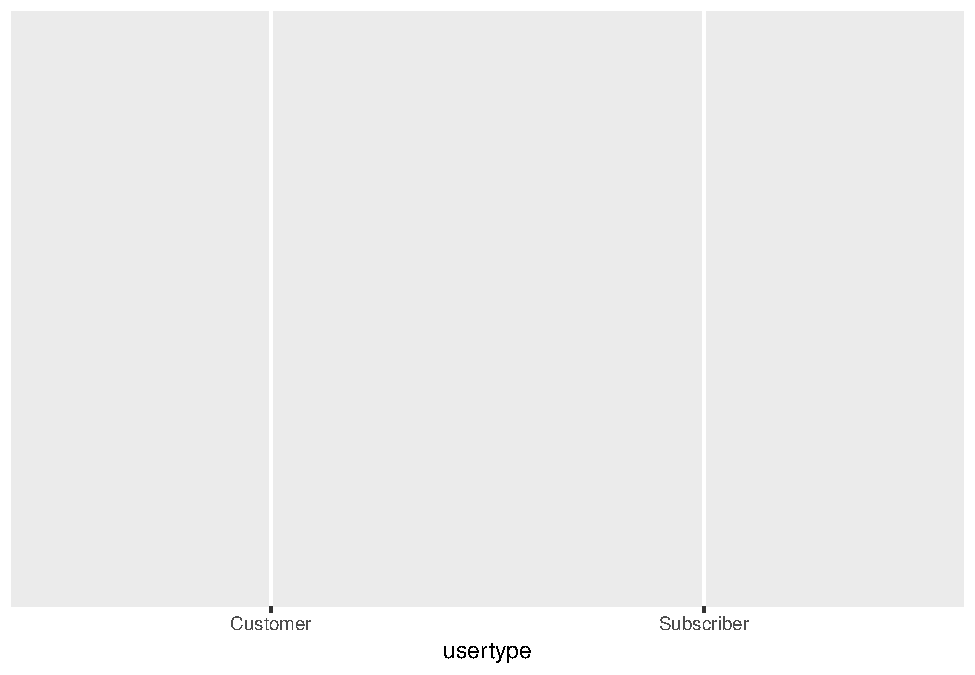
\includegraphics{met-council-introR_files/figure-latex/unnamed-chunk-30-1.pdf}

\textbf{Stage 3}: Add some shapes

\begin{Shaded}
\begin{Highlighting}[]
\KeywordTok{ggplot}\NormalTok{(nice_ride_}\DecValTok{2018}\NormalTok{, }\KeywordTok{aes}\NormalTok{(}\DataTypeTok{x =}\NormalTok{ usertype)) }\OperatorTok{+}\StringTok{ }
\StringTok{  }\KeywordTok{geom_bar}\NormalTok{() }\CommentTok{# add the geoms}
\end{Highlighting}
\end{Shaded}

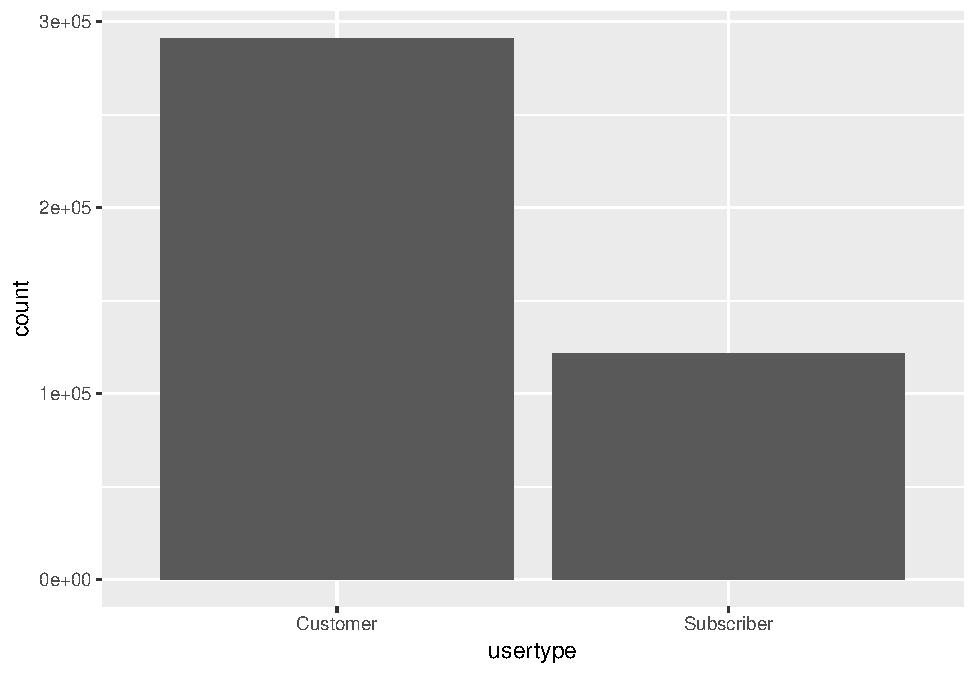
\includegraphics{met-council-introR_files/figure-latex/unnamed-chunk-31-1.pdf}

\textbf{Stage 4}: Give your plot a title

\begin{Shaded}
\begin{Highlighting}[]
\KeywordTok{ggplot}\NormalTok{(nice_ride_}\DecValTok{2018}\NormalTok{, }\KeywordTok{aes}\NormalTok{(}\DataTypeTok{x =}\NormalTok{ usertype)) }\OperatorTok{+}\StringTok{ }
\StringTok{  }\KeywordTok{geom_bar}\NormalTok{() }\OperatorTok{+}
\StringTok{  }\KeywordTok{labs}\NormalTok{(}\DataTypeTok{title =} \StringTok{"User Types"}\NormalTok{) }\CommentTok{# add a title}
\end{Highlighting}
\end{Shaded}

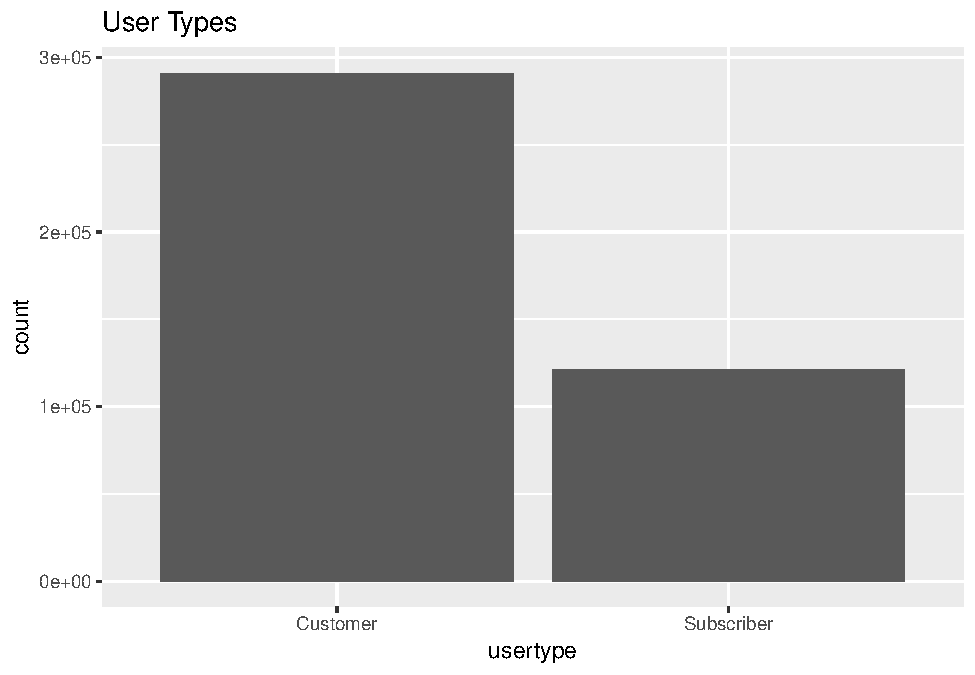
\includegraphics{met-council-introR_files/figure-latex/unnamed-chunk-32-1.pdf}

Now we have a plot! There are many ways to customize it, but for now
this is a great start.

\subsection{Try it out}\label{try-it-out-2}

Let's create a plot of the bike types (\texttt{bike\_type}).

\textbf{Stage 1}: The plotting canvas

\begin{Shaded}
\begin{Highlighting}[]
\KeywordTok{___}\NormalTok{(nice_ride_}\DecValTok{2018}\NormalTok{) }\CommentTok{# set up our plotting area }
\end{Highlighting}
\end{Shaded}

\textbf{Stage 2}: Frame your data with axes

\begin{Shaded}
\begin{Highlighting}[]
\KeywordTok{___}\NormalTok{(nice_ride_}\DecValTok{2018}\NormalTok{, }\KeywordTok{___}\NormalTok{(}\DataTypeTok{x =}\NormalTok{ ___)) }\CommentTok{# set up our axes}
\end{Highlighting}
\end{Shaded}

\textbf{Stage 3}: Add some shapes

\begin{Shaded}
\begin{Highlighting}[]
\KeywordTok{___}\NormalTok{(nice_ride_}\DecValTok{2018}\NormalTok{, }\KeywordTok{___}\NormalTok{(}\DataTypeTok{x =}\NormalTok{ ___)) }\OperatorTok{+}\StringTok{ }
\StringTok{  }\KeywordTok{geom____}\NormalTok{() }\CommentTok{# add the geoms}
\end{Highlighting}
\end{Shaded}

\textbf{Stage 4}: Give your plot a title

\begin{Shaded}
\begin{Highlighting}[]
\KeywordTok{___}\NormalTok{(nice_ride_}\DecValTok{2018}\NormalTok{, }\KeywordTok{___}\NormalTok{(}\DataTypeTok{x =}\NormalTok{ ___)) }\OperatorTok{+}\StringTok{ }
\StringTok{  }\KeywordTok{geom____}\NormalTok{() }\OperatorTok{+}
\StringTok{  }\KeywordTok{___}\NormalTok{(}\DataTypeTok{title =}\NormalTok{ ___) }\CommentTok{# add a title}
\end{Highlighting}
\end{Shaded}

Does your plot look like this?

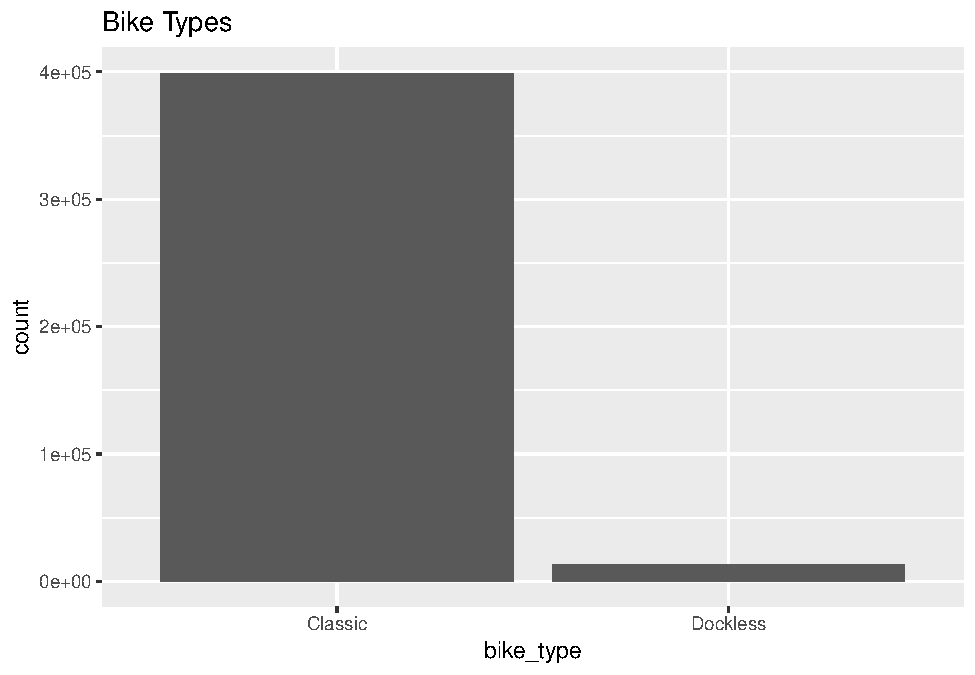
\includegraphics{met-council-introR_files/figure-latex/unnamed-chunk-37-1.pdf}

\subsection{Quantitative data}\label{quantitative-data}

\chapter{Data Wrangling}\label{data-wrangling}

\chapter{Visualization, revisited}\label{visualization-revisited}

\chapter{Modeling}\label{modeling}

\chapter{Reading in data, revisited}\label{reading-in-data-revisited}

\chapter{More resources}\label{more-resources}

\chapter{Miscellaneous notes}\label{miscellaneous-notes}

\bibliography{book.bib,packages.bib}


\end{document}
